\documentclass{article}
\usepackage[utf8]{inputenc}
\usepackage{graphicx}
\usepackage{epstopdf}
\usepackage{caption}
\usepackage{subcaption}
\usepackage{multirow}
\usepackage{hyperref}
\usepackage{url}
\usepackage{seqsplit}
\hypersetup{pdfstartview={FitH null null null}}
\usepackage{amssymb,amsmath}
\usepackage{amsthm}
\usepackage{empheq}
\usepackage{algorithm,algpseudocode}
\usepackage[margin=1.5in]{geometry}
\usepackage{listings}
\usepackage{program}
\usepackage{commath}
\lstset{language=Python} 

\usepackage{listings}
\usepackage{color} %red, green, blue, yellow, cyan, magenta, black, white
\definecolor{mygreen}{RGB}{28,172,0} % color values Red, Green, Blue
\definecolor{mylilas}{RGB}{170,55,241}


\title{Computational Modeling of Molecular Structures}
%\subtitle{A snapshot of the current state-of-the-art in Bioinformatics}
\author{Caiwei Wang, Xiaokai Qian, Sean Lander, \\Haipei Fan, Puneet Gaddam, Brett Koonce\\\\University of Missouri - Columbia}

\date{May 12, 2014}

\algloopdefx{NoEndIf}[1]{\textbf{If} #1 \textbf{then}}

\begin{document}

\maketitle

\begin{abstract}

With the advancement of technology, and a growing interest in computational methods, new fields are being created on an almost daily basis in order to utilize the new power that is now at hand. One field in which this move has had one of the largest impacts has been Biology with the creation of Bioinformatics, with major strides being made in genetics in particular. Over the past two decades movement in this field, specifically in learning and predicting the three-dimensional models of proteins and chromosomes, has lead to incredible discoveries and rapid advancements in medicine and genetic modification. In order to better understand this field we have experimented with and implemented current state of the art methods and technologies available to these fields in order to assess their abilities and better sense what the future of biological studies may hold.

\end{abstract}

\section{Introduction}

Proteins, from the smallest amoeba to the largest living organisms, are the building blocks of all life on our planet.  With the advent of modern sequencing techniques, we possess a copy of these organism's (and our own) genetic code.  Deep within the ribosome, cells within continually build new proteins from DNA.  Given the same blueprint, though, we cannot accurately model what Mother Nature does so easily.\\\\
Molecular structures obey the laws of nature.  In theory, we are masters of the atom: we have enough knowledge of physics, chemistry and math to be able to predict any interaction correctly.  But, in practice, biology remains frustratingly difficult to quantify.  With modern machines we can perform a billion simulations in the blink of an eye but still cannot accurately replicate what a single protein knows how to do with nothing more than its very own DNA sequence.\\\\
Some of this is because our tools, be they computers or algorithms, are still relatively limited.  Computational modeling of molecular structures is a very, very new field.  Every field starts in this way, however, and thus it is important to take record of the technologies introduced and implemented from the beginning in order to lead the direction of the field. With this in mind we will present to the reader a snapshot of the curent state-of-the-art technologies in the field of Bioinformatics used in the modeling of DNA-based molecular structures, from proteins to the genome. We start with what is relatively the oldest modeling technique, Template Based Modeling for protein structures, and move forward in time to Template Free Modeling, onto Protein Docking prediction methods, and finally Chromosome conformation prediction, an area which is currently less than a decade old yet moving forward at a rapid pace.


\section{Methods and Implementation}

\subsection{Template Based Protein Modeling}

Template Based Modeling centers around creating the structure of the target protein using the structure of a protein with a similar sequence as a template. Using a template structure and its alignment with the target we are able to confidently create a structure for the target which is close to native. After building a initial structure for the target, we can use existing tools to refine our model.

%\begin{center}
%	\subsubsection*{Template Based Modeling Pipeline}
%		\begin{figure}[H]
%		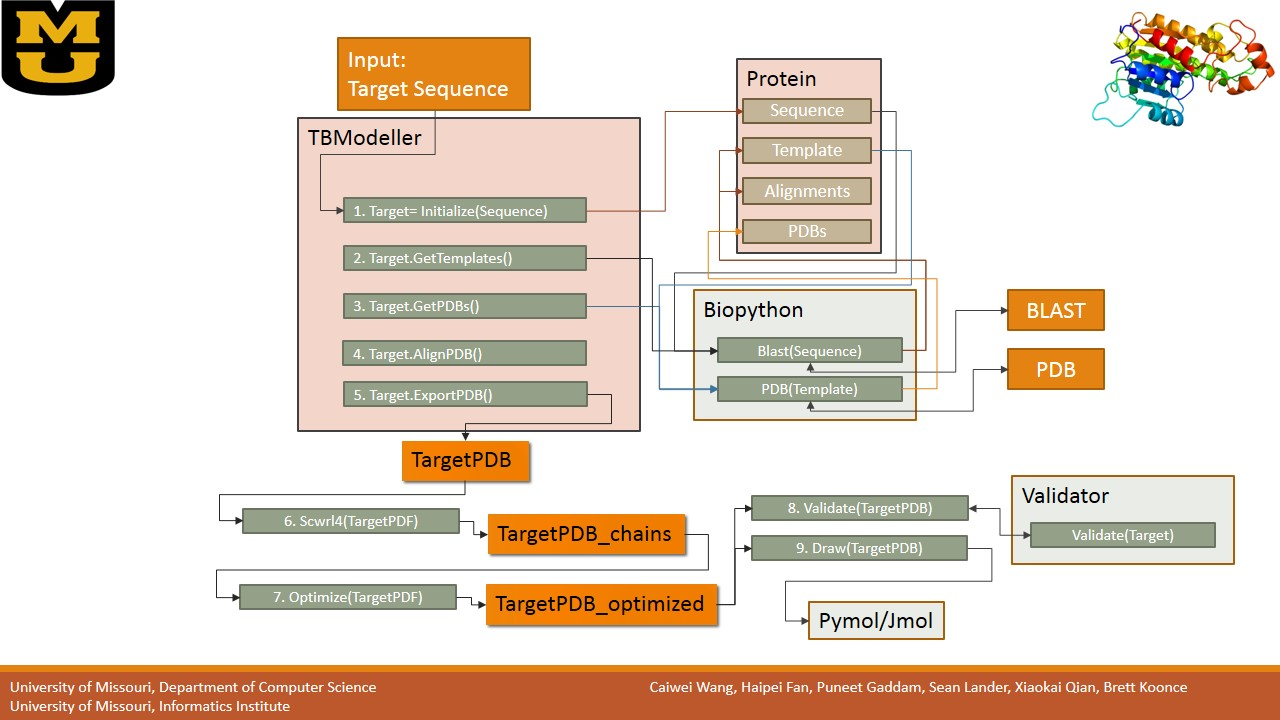
\includegraphics[width=\textwidth]{TBM-pipeline}
%		\caption{An overview of the TBPy pipeline}
%		\label{Fig:tbmpipeline}
%		\end{figure}
%\end{center}

\subsubsection{Building a Decoy}

\subsubsection*{PDB to Structure}

The structure is created by using an alignment file and a structure file to create a structure for the target. Under optimal circumstances there will be no difference in length between the target and template. However this is not always the case, so it is important to pad the front and back of the template's alignment and structure with blank residues. This is recorded as a single dash, -, in the alignment and a triple dash, - - -, in the structure. The structure is preprocessed and reduced down to a series of residues, each containing 4 atoms: N, CA, C, O. Residue names are changed from length 3 to length 1 so as to facilitate alignment checking between the template's alignment and structure.


\subsubsection*{Structure to PDB}

Once the preprocessing is complete the alignment and structure can be used to create the target's structure. The basic idea is:
A) If the residue of the target is aligned with a residue of the template, copy its coordinates to the residue of the target. 
B) If one residue of the target is blank in the alignment file, skip it and go on next one.
C) If the residue of the target is non-blank and the residue of the template is blank in the alignment file, create a blank residue for this target’s residue.


\subsubsection{Optimization}


\subsubsection*{Loop Modeling - MODELLER}

First, there are still gaps in our protein where the two structures did not match. In these spots, our script generates matching protein data, but these atoms are simply generated and as such not part of the final protein. To combat this problem, we have modified our code slightly to output missing residues. Then, we use Modeller, a popular python tool in protein modeling, to re-optimize these residues so that they will match the rest of our protein.


\subsubsection*{Side-chain Modeling - SCXWRL4}

Next, we run our candidate PDB file through SCWRL, a program for optimizing the side chains in our protein backbone. SCWRL4 is based on an improved graph theory algorithms that solve the combinatorial problem in side-chain prediction more rapidly than many other available programs.\\\\
SCWRL4 is based on a new potential function that results in improved accuracy at reasonable speed.It will converge on very large proteins or protein complexes or those with very dense interaction graphs.It depends on a backbone-dependent rotamer library. The library provides lists of chi1-chi2-chi3-chi4 values and their relative probabilities for residues at given phi-psi values, and explores these conformations to minimize sidechain-backbone clashes and sidechain-sidechain clashes.\\\\
The SCWRL4 executable saves the resolved optimal conformation of the whole protein model into PDB file. The corresponding value of the total energy is printed into the standard output, which can be redirected to a file for further analysis.


\subsubsection*{Refinement - 3DRefine}

Finally, we used a two-step refinement protocol, called 3Drefine, to consistently bring the initial model closer to the native structure. One of the major limitations of computational protein structure prediction is the deviation of predicted models from their experimentally derived true, native structures. The first step is based on optimization of hydrogen bonding (HB) network and the second step applies atomic-level energy minimization on the optimized model using a composite physics and knowledge-based force elds. The approach has been evaluated on the CASP benchmark data and it exhibits consistent improvement over the initial structure in both global and local structural quality measures. 3Drene method is also computationally inexpensive, consuming only few minutes of CPU time to refine a protein of typical length (300 residues).


\subsection{Template Free Modeling}

Template free modeling is an important technique in modern bioinformatics since many proteins do not have good templates to base a computational model on. First, we begin with PDB sequences converting into torsion angles using third party tools RAMA/LIPA (part of CRONKITE). Using a sliding window algorithm, we can add millions of fragments to our database. Then, for each segment, we can do a query for a match/similar protein in the database.\\\\
We use the neighbor's energy as a score, and when the current solution’s neighbor is better it is accepted. If not, we select the neighbor with a probability based on the current temperature. For our project, we implemented a basic homology modeling pipeline in python, using a number of external tools like dFire, PyMOL and TM-score to build/present a final visualized model.

%\begin{center}
%	\subsubsection*{Template Free Modeling Pipeline}
%	\begin{figure}[H]
%	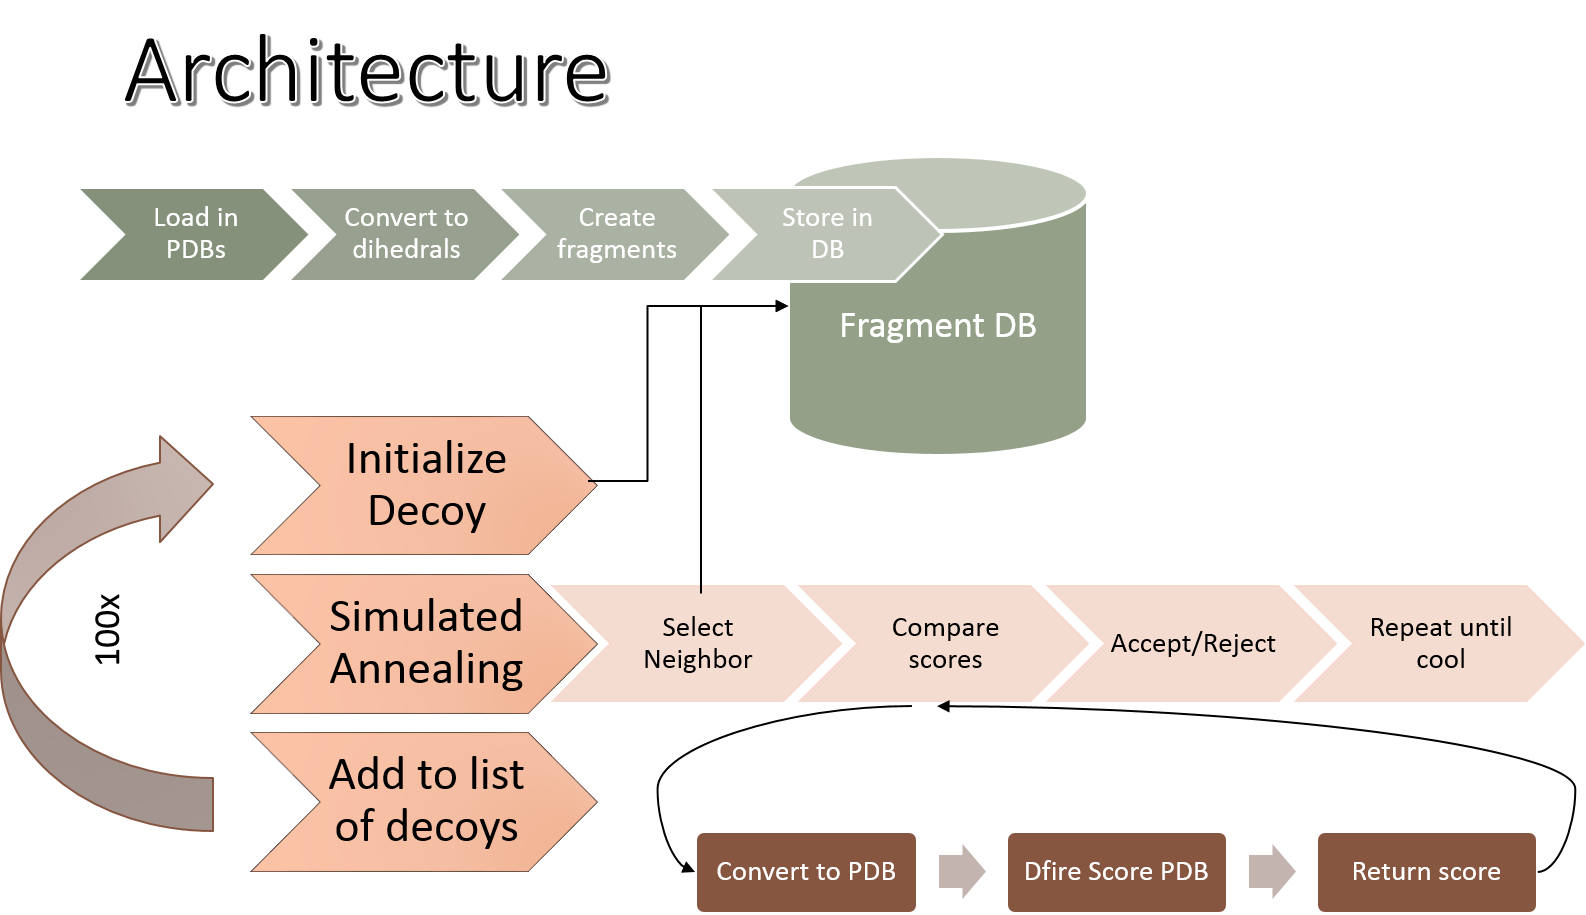
\includegraphics[width=\textwidth]{TFM-pipeline}
%	\caption{An overview of the TFPy pipeline}
%	\label{Fig:tfmpipeline}
%	\end{figure}
%\end{center}

In order to more easily assemble our workflow we break it into a simple pipeline. Doing this allows for quick iteration on multiple fronts without the fear of breaking the model as a whole.\\\\
Creating a system in this way leads to easy parallelization, as each decoy can be generated independent of the others. This allows for rapid decoy creation and comparison with no human component necessary beyond initial input.


\subsubsection{Fragment Database}

First, we selected a set of 17,000 PDB database with sequence lengths of 100-150 residues from an internal collection at MU.  For each PDB file, we split it into a list of (residue, phi angle, psi angle) chunks.  We discard the first and last residue, since they only have one valid angle.  First, we go through each PDB file sequentially for each sequence of three residues, then again for each sequence of nine residues.


\subsubsection{Simulated Annealing}

After building our fragments database, we build a initial model of our target using sequences from the database. Then, to improve our model, we use simulated annealing, a generic probabilistic metaheuristic for the global optimization problem of locating a good approximation to the global optimum of a given function in a large search space. It is often used when the search space is discrete and can prove quite efficient. Unlike hill climbing, simulated annealing can allow a poorer fragment replacement (a weaker score) early on when the function has a high temperature, which often leads to a better overall model structure.\\\\
In each cycle, we build a random neighbor of the current best solution. If the neighbor’s score is better, we promote it to  the current solution. Otherwise, we select one of the two with a probability based on the current global temperature.  Allowing a “bad” fragment replacement can allow the SA algorithm to avoid local optima.


\subsubsection{Neighbor Selection}

\subsubsection*{BLOSUM62}

Neighbor selection is an important part of greedy and semi-greedy algorithms, as changes which are too large can disrupt the process of finding global minima and maxima. In order to generate neighbors which are close to the current sequence we use a two-fold approach: find a complete match; if a match is not found, find a match for a very similar sequence. The first approach is easy to understand, but the second requires domain knowledge of amino acids, as some acids are more similar than others.

\begin{equation*}
	S_{ij}= \left( \frac{1}{\lambda} \right)\log{\left( \frac{p_{ij}}{q_i * q_j} \right)}
\end{equation*}

The Blosum62 matrix is a pair-wise "distance" matrix of sorts which can be used to determine the similarity of two amino acids. This matrix is commonly used to determine sequence similarity for alignment purposes, but can also be used as a generative model. By finding similar amino acids to those in the current fragment sequence, we can generate multiple sequences which are very similar in terms of "distance," allowing us to expand our search criteria on limited databases.


\subsubsection*{Scoring with dFire Energy}

To provide an objective score of our new protein for the purposes of picking which model to accept, we use dFire energy.  The dFire-based statistical potential is a more physically accurate potential than other all-atom statistical potentials because the potential satisfies the physical requirement that the same water-mediated interaction between amino acid residues is responsible for folding and binding. This potential is more accurate for longer loops (9 to 12 residues). The performance of the dFire potential for loop selections is useful as well because the computational cost of a statistical potential is only a fraction of what is needed for physical-based energy functions with implicit solvation models. As such, a single-term dFire-statistical energy function can provide an accurate loop prediction at a fraction of computing cost required for more complicate physical-based energy functions.


\subsection{Protein Docking}

Protein-protein docking is used to predict the structure of a protein complex given a receptor and a ligand. It is very useful in drug creation and disease prevention. Because the computational power needed for predictions can be high, many unique algorithms and methods have been created to both predict and score docked structures.\\\\
For this method comparison we will be using three prediction servers, each of which use a variation on the Fast Fourier Transform method for prediction and their own unique methods for rankings. We then standardize these predictions using RosettaDock's scoring function. Once the top 10 are selected we will apply Rosetta's optimization method, which allows for a relaxing of side-chain constraints, before scoring and sorting them a second time. We will then use RMSD, a traditional scoring method when native conformation is known, of the predicted interface in order to analyze and compare the different methods of prediction, optimization, and scoring.

%\begin{center}
%	\subsubsection*{Protein Docking Pipeline}
%	\begin{figure}[H]
%	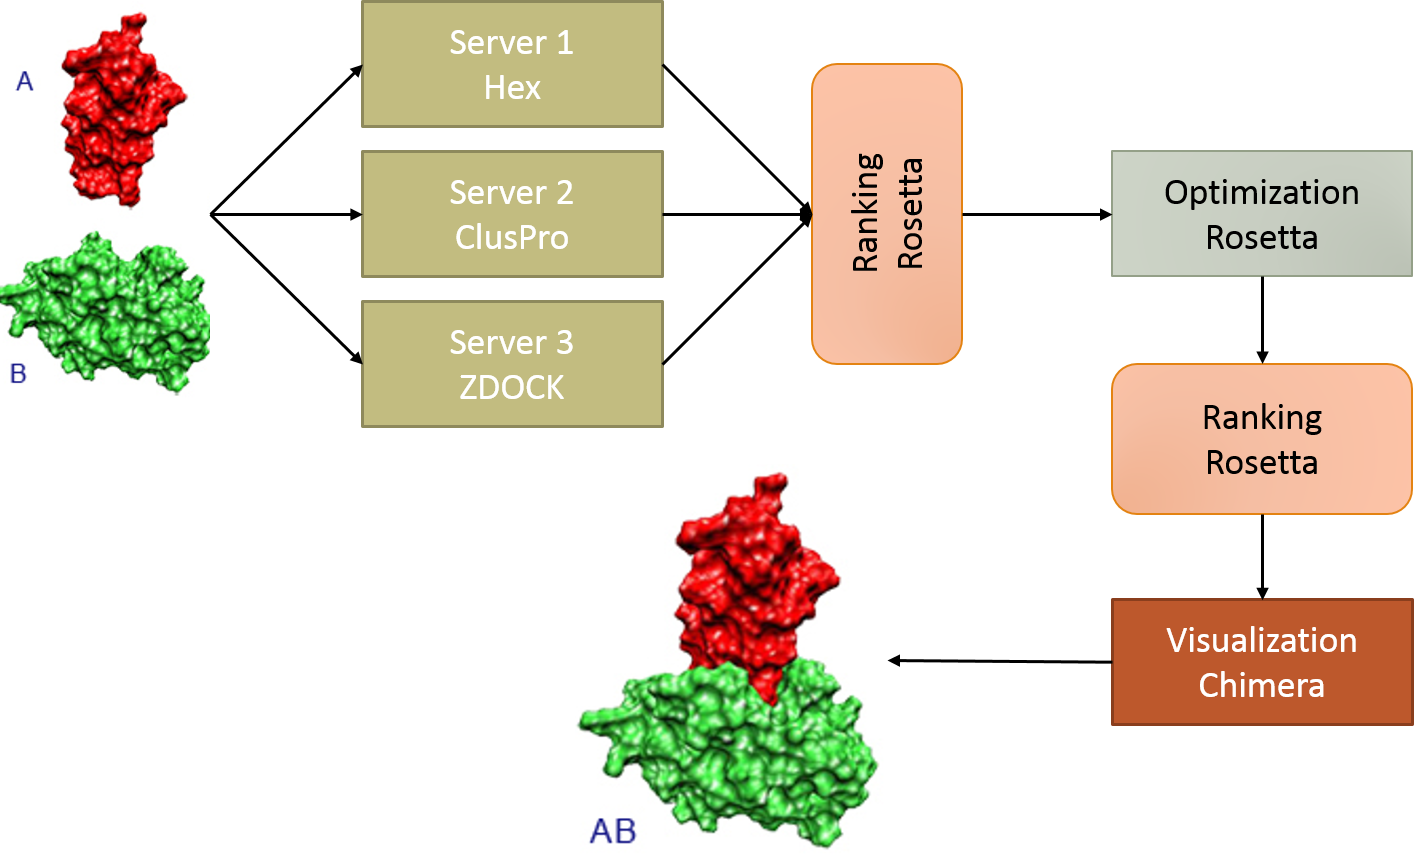
\includegraphics[width=\textwidth]{PD-pipeline}
%	\caption{An overview of the protein docking pipeline}
%	\label{Fig:pdpipeline}
%	\end{figure}
%\end{center}

\subsubsection{Protein Docking Tools}

\subsubsection*{Hex}

Hex server is the first Fourier transform (FFT)-based protein docking server to be powered by graphics processors. Using two graphics processors simultaneously, a typical 6D docking run takes approximately 15 s, which is up to two orders of magnitude faster than conventional FFT-based docking approaches using comparable resolution and scoring functions. The server requires two protein structures in PDB format to be uploaded, and it produces a ranked list of up to 1000 docking predictions. Knowledge of one or both protein binding sites may be used to focus and shorten the calculation when such information is available. The first 20 predictions may be accessed individually, and a single file of all predicted orientations may be downloaded as a compressed multi-model PDB file. The server is publicly available and does not require any registration or identification by the user.


\subsubsection*{ClusPro}

ClusPro is a web server which uses an automated rigid-body docking and discrimination algorithm that rapidly filters docked conformations, and ranks them based on their clustering properties.\\\\
After signing up for an account and logging into the server, you can create a docking job with a receptor and ligand by uploading the PDB files of T50 and T53. You may optionally choose what chains to use in docking. After that, you can view the queue status for the decoys completed. It will generate the number of top models you choose.


\subsubsection*{ZDOCK}

ZDOCK uses a mixture of Fast Fourier Transform and data-driven scoring/ranking in order to create and sorts its decoy. While this allows for very fast decoy creation, it results in a stochastic algorithm, so multiple runs will always generate the same results. The ZDOCK server produces 500 decoys on a run, but only the top 10 of those are available for download, making it hard to build up an appropriately sized sample group.


\subsection{Chromosome Modeling}

The human genome has been sequenced, but modelling the human chromosome remains a difficult task.  One promising avenue of modern research lies in the technique of Hi-C sequencing, which produces contact maps as part of the sequencing process.  By analyzing which regions of the genome are often found together, we can build up a map of the larger genome.  Trieu and Cheng recently proposed a new method based on an objective function that promises to be able to build a model using gradient descent from the Hi-C data.  We decided to put their results to the test, as well as experiment with solving the objective function using stochastic (MCMC and SA) methods.

%\begin{center}
%	\subsubsection*{Chromosome Modeling}
%	\begin{figure}[H]
%	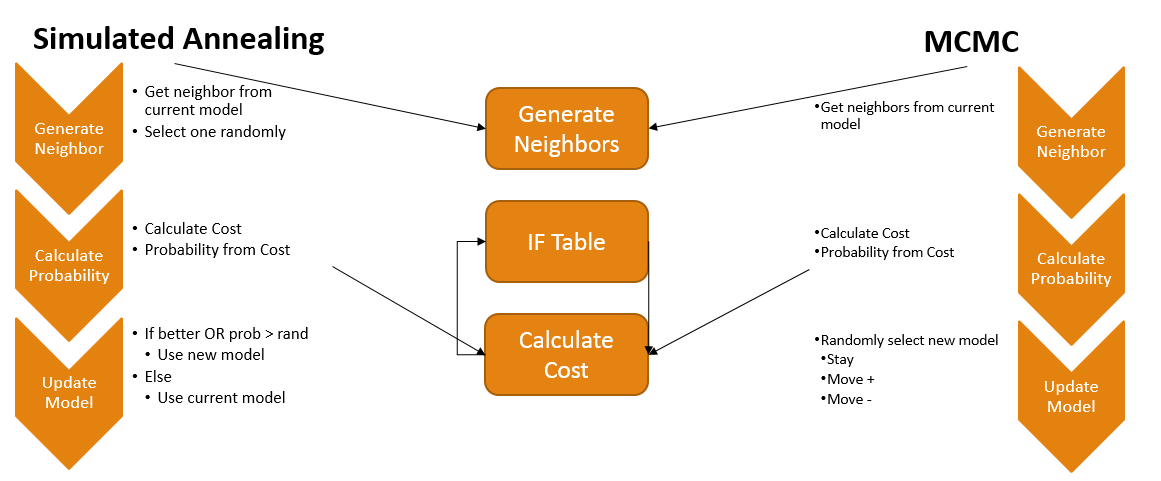
\includegraphics[width=\textwidth]{CM-pipeline}
%	\caption{An overview of the chromosome modeling}
%	\label{Fig:cmpipeline}
%	\end{figure}
%\end{center}

\subsubsection{Objective function}

Simply put, the objective function advanced by Trieu and Cheng can be expressed as follows:

\begin{equation}
      TotalModelScore(m) = ContactScore(m) + NonContactScore(m) + PairSmoothing(m)
\end{equation}

The first operation minimizes the distances of contacts with affinity to keep them in contact (but keeps their distance above a minimum threshold):

\begin{equation}
      ContactScore(m) = \sum_{i=1}^{n} \sum_{j=1}^{n} (\abs{i-j}>1) * (W_1 * \tanh(d_c^2-d_{ij}^2) * N_{ij} + W_2 * \tanh(d_{ij}^2-d_{min}^2))
\end{equation}

The second operation maximizes the distances of contacts without affinity to keep them away from contact (but keeps their distance below a maximum threshold):

\begin{multline}
      NonContactScore(m) = \sum_{i=1}^{n} \sum_{j=1}^{n} (\abs{i-j}>1) * (W_3 * \tanh(d_{max}^2-d_{ij}^2) / TotalIF \\+ W_4 * \tanh(d_{ij}^2-d_{c}^2) / TotalIF)
\end{multline}

The third operation tweaks the scores of consecutive contacts slightly so that moving them is favored over adjusting more distant relationships:

\begin{multline}
      PairSmoothing(m) = \sum_{i=1}^{n} \sum_{j=1}^{n} (\abs{i-j}=1) * (W_1 * IF_{max} / TotalIF * \tanh(da_{max}^2-d_{ij}^2) \\+ W_2 * \tanh(d_{ij}^2-d_{min}^2) / TotalIF)
\end{multline}

We also used the following table of constants from Trieu and Cheng's paper.  They are experimentally derived values.

\begin{center}
\begin{tabular}{|l|c|c|c|r|}
\multicolumn{4}{c}{Constants} \\
    \hline
    $d_{min}$ & $\sqrt 0.2$ & W1 & 1.0           \\ \hline
    $d_{max}$ & 4.5  & W2 & 1.5      \\ \hline
    $d_{c}$ & $\sqrt 7.0$  & W3 & 1.5            \\ \hline
    $da_{max}$ & $\sqrt 1.8$  & W4 & 1.5     \\ \hline
    \end{tabular}
\end{center}

We also make use of the following:

\begin{equation}
      TotalIF = \sum_{i=1}^{n} \sum_{j=1}^{n} IF(i,j)
\end{equation}

\begin{equation}
      N(i,j) = IF(i,j)/TotalIF
\end{equation}

\begin{equation}
      IF_{max} = \max(IF(i,j),IF(j,i))
\end{equation}

Combining the above equations, we end up with a combined objective function of approximately 50000 subproblems, as detailed above.  Our problem now is simply to maximize the result given a 471 variable input vector (157 contacts * 3 coordinates $(x, y, z)$) across this space.  Towards this end, we present one deterministic and two stochastic methods of optimization.  For each version, our initial solution subspace is randomly chosen coordinates in the domain $-0.5 \leq (x, y, z) \leq 0.5$.

\subsubsection{Simulated Annealing}

For our first test of stochastic methods, we built a simulated annealer capable of solving our objective function.  SA is a well known non-deterministic algorithm to sample a state space quickly.  Essentially, we start from a random model, then generate a neighboring model (our original model with a modification).  We score the two models.  If the new one is better, we accept it, otherwise we only replace our existing model based on a gradually decreasing schedule (temperature function).  As such, the two most important parts of implementing simulated annealing are the temperature function and how we generate neighbor models.


\subsubsection{Markov-Chain Monte Carlo (MCMC)}

For our second test of stochastic methods, we built a Markov-Chain Monte Carlo sampler.  Markov chains are an important technique in computer science from statistics.  First, we build up a graph model of discreet events with a corresponding transition matrix.  Next, we seed the transition matrix using real-world data (generally derived from posterior probability distributions).  Then, we can sample the Markov model repeatedly (Monte Carlo) to try and converge upon a solution space that is generally an excellent model of our problem domain.\\\\
For our project, we utilized MCMC to optimize our state/input vector (coordinate data) to most closely approximate our posteior distribution (our objective function).  Our methods converged well, but required some time to mix (~600k simulations).  We utilized a different neighborhood function than we used in Simulated Annealing.  First, we select a random region from which to generate a neighborhood. The neighborhood is then created by increasing/decreasing the location in each of the three dimensions: $(x, y, z)$. In this way we generate 8 neighbors and a default position which are scored and given a probability of selection based on the score range, with higher scoring conformations more likely to be sampled. Once a new neighbor conformation is selected the process repeats until all iterations have completed.


\section{Results}

\subsection{Template Based Modeling}

After we obtain our final target PDB file, we use Jmol to visualize it. At the same time, we also visualize the native one to compare it with our prediction. The left one is a target structure we generated (T0644), while right one is the native structure.\\\\


%\begin{center}
%	\subsubsection*{Native and Decoy}
%	\begin{minipage}{.5\textwidth}
%	  \centering
%	  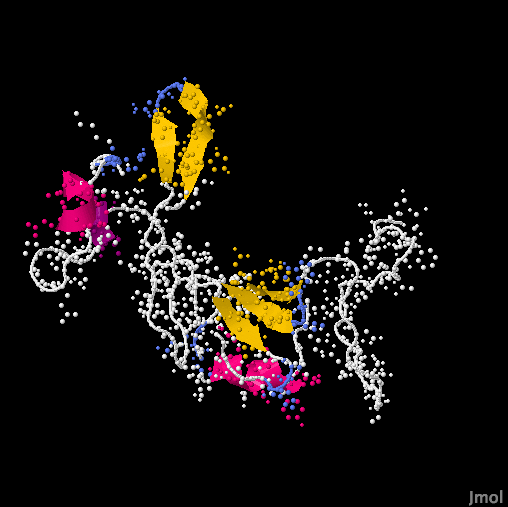
\includegraphics[width=.9\linewidth]{TBM-target_group_v2}
%	  \captionof{figure}{Target structure}
%	  \label{fig:tbm-decoy}
%	\end{minipage}%
%	\begin{minipage}{.5\textwidth}
%	  \centering
%	  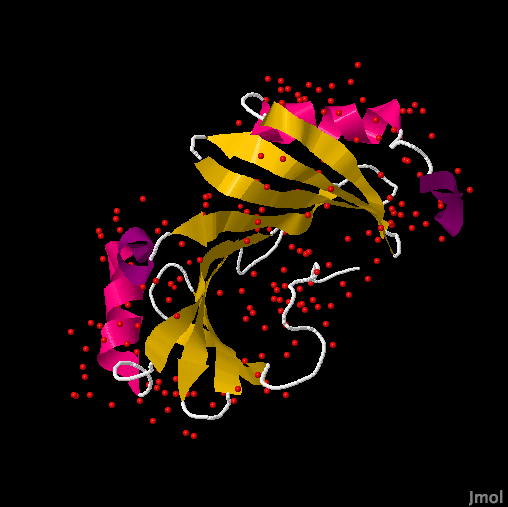
\includegraphics[width=.9\linewidth]{TBM-target_native}
%	  \captionof{figure}{Native structure}
%	  \label{fig:tbm-native}
%	\end{minipage}
%\end{center}

After we generate the target PDB file, we use TM-Score and RMSD to evaluate our prediction. Also, we compared our prediction with other servers' results based on same target. For our project, we choose MuFold and MULTICOM to provide a benchmark.


\begin{center}
	\subsubsection*{Scores}
    \begin{tabular}{ | l | l | l | p{2cm} |}
    \hline
      & Group1 & MULTICOM & MuFold \\ \hline
    TM-Score & 0.9971 & 0.9072 & 0.1985 \\ \hline
    RMSD & 0.23 & 1.666 & 14.978 \\
    \hline
    \end{tabular}
\end{center}


\subsection{Template Free Modeling}

As before, our targets were: T0693 (100 residues), T0666 (196 residues), and T0695 (537 residues).  Each score contains the best result from the 9-sequence replacement pass, followed by the score from the best 3-sequence replacement pass.

\begin{center}
\begin{tabular}{|l|c|c|c|r|}
\multicolumn{5}{c}{T0693} \\
    \hline
      & Linear - 9 & Linear - 3 & Sigmoid - 9 & Sigmoid - 3\\ \hline
    dDFIRE & -175.6 & -177.39 & -180.98 & -194.71 \\ \hline
    TM-Score & 0.0891 & 0.0745 & 0.1162 & 0.0908 \\ \hline
    RMSD & 16.856 & 16.868 & 14.447 & 14.554 \\
    \hline
    \end{tabular}
\end{center}

\begin{center}
\begin{tabular}{|l|c|c|c|r|}
\multicolumn{5}{c}{T0666} \\
    \hline
      & Linear - 9 & Linear - 3 & Sigmoid - 9 & Sigmoid - 3\\ \hline
    dDFIRE & -75.27 & -121.34 & -82.85 & -125.35 \\ \hline
    TM-Score & 0.16113 & 0.162 & 0.1779 & 0.1565 \\ \hline
    RMSD & 23.162 & 22.569 & 25.193 & 30.457 \\
    \hline
    \end{tabular}
\end{center}

\begin{center}
\begin{tabular}{|l|c|c|c|r|}
\multicolumn{5}{c}{T0695} \\
    \hline
      & Linear - 9 & Linear - 3 & Sigmoid - 9 & Sigmoid - 3\\ \hline
    dDFIRE &  -372.27 & -375.93 & -425.11 & -431.09 \\ \hline
    TM-Score & 0.1061 & 0.1362 & 0.13 & 0.119 \\ \hline
    RMSD & 36.765 & 37.403 & 39.106 & 41.541 \\
    \hline
    \end{tabular}
\end{center}


\subsection{Protein Docking}

\subsubsection*{Non-optimized Scores}

After we generate decoys from three servers, we pick the best decoy as our evaluation target. We use TM-score and RMSD(overall) as our score functions. The following are our two result tables:

\begin{center}
\begin{tabular}{|l|c|c|c|r|}
\multicolumn{4}{c}{T50} \\
    \hline
      & ClusPro & ZDock & Hex \\ \hline
    TM-Score & 0.9941 & 0.1490 & 0.9941 \\ \hline
    RMSD & 0.541 & 25.304 & 0.514 \\
    \hline
    \end{tabular}
\end{center}

\begin{center}
\begin{tabular}{|l|c|c|c|r|}
\multicolumn{4}{c}{T53} \\
    \hline
      & ClusPro & ZDock & Hex \\ \hline
    TM-Score & 0.2418 & 0.8420 & 0.2418 \\ \hline
    RMSD & 8.712 & 16.637 & 8.712 \\
    \hline
    \end{tabular}
\end{center}


\subsubsection*{Optimized Scores}

After that, we used Rosettadock to optimize our decoys from three servers. Since the format of ZDock results is not acceptable for Rossettadock, we only optimize decoys of Hex and Cluspro. The next two table show these results (we only present the top structure). Very interesting, there is no improvement. We may figure out this problem in further work.

\begin{center}
\begin{tabular}{|l|c|c|c|r|}
\multicolumn{3}{c}{T50} \\
    \hline
      & ClusPro & Hex \\ \hline
    TM-Score & 0.9941 & 0.9941 \\ \hline
    RMSD & 0.514 & 0.514 \\
    \hline
    \end{tabular}
\end{center}

\begin{center}
\begin{tabular}{|l|c|c|c|r|}
\multicolumn{3}{c}{T53} \\
    \hline
      & ClusPro & Hex \\ \hline
    TM-Score & 0.2418 & 0.2418 \\ \hline
    RMSD & 8.712 & 8.712 \\
    \hline
    \end{tabular}
\end{center}


\subsubsection*{Interface Scores}

Since overall rmsd can not reflect the quality of the complex very well, we tried to compare the interfaces of decoys with the one of native structure. The next two tables show results. From these two tables, they indicate that good overall RMSD can’t promise a good interface structure.

\begin{center}
\begin{tabular}{|l|c|c|c|r|}
\multicolumn{4}{c}{T50} \\
    \hline
      & ClusPro & ZDock & Hex \\ \hline
    TM-Score & 0.1890 & 0.0291 & 0.1920 \\ \hline
    RMSD & 0.328 & 20.319 & 0.334 \\
    \hline
    \end{tabular}
\end{center}


\begin{center}
\begin{tabular}{|l|c|c|c|r|}
\multicolumn{4}{c}{T53} \\
    \hline
      & ClusPro & ZDock & Hex \\ \hline
    TM-Score & 0.0592 & 0.0979 & 0.0557 \\ \hline
    RMSD & 2.894 & 3.854 & 3.858 \\
    \hline
    \end{tabular}
\end{center}


\subsection{Chromosome Modeling}

\begin{center}
\begin{tabular}{|l|c|c|c|r|}
\multicolumn{2}{c}{Iterations/minute} \\
    \hline
    SA & 10,000 \\ \hline
    MCMC: greedy & 1750    \\ \hline
    MCMC: non-greedy & 1700    \\ \hline
    \end{tabular}
\end{center}


\section{Conclusion}

From the above tests it is apparent that, while some methods point in the right direction, work in this area is far from over and ripe for discovery. Standardization is necessary for cross-tool compatibility, first off, and much more data is needed in order to fully utilize the most successful data-driven approaches. For stochastic methods, more accurate scoring methods are needed, using knowledge from fields spanning statistical theory to physics and chemistry, and, most importantly, the microbiologists currently working in crystalography and high-accuracy imaging. This continues to be a young and developing field waiting for its equivalent of merge-sort, but thanks to the energy and excitement surrounding its potential that is likely to come sooner rather than later.


\section{Citations}

We thank the following tools and papers: \\

\begin{enumerate}

\item Cock PJ, Antao T, Chang JT, Chapman BA, Cox CJ, Dalke A, Friedberg I, Hamelryck T, Kauff F, Wilczynski B, and de Hoon MJ. Biopython: freely available Python tools for computational molecular biology and bioinformatics. Bioinformatics 2009 Jun 1; 25(11) 1422-3.

\item Blast:  Altschul S.F., Gish W., Miller W., Myers E.W. and Lipman D.J. (1990)
Basic local alignment search tool.  J. Mol. Biol. 215: 403-410.

\item CASP: Critical Assessment of Techniques for Protein Structure Prediction. http://predictioncenter.org/casp10/

\item D.W.Heinz, W.A.Baase, F.W.Dahlquist, B.W.Matthews, "How Amino-Acid Insertions are Allowed in an Alpha-Helix of T4 Lysozyme," Nature, 361 (1993): 561.

\item D. Bhattacharya and J. Cheng: 3Drefine: Consistent Protein Structure Refinement by Optimizing Hydrogen-Bonding Network and Atomic-Level Energy Minimization.
Proteins: Structure, Function and Bioinformatics. 2012 (In Press).

\item G. G. Krivov, M. V. Shapovalov, and R. L. Dunbrack, Jr. Improved prediction of protein side-chain conformations with SCWRL4. Proteins (2009).

\item Jmol: an open-source Java viewer for chemical structures in 3D. http://www.jmol.org/ 

\item PyMOL: http://sourceforge.net/projects/pymol/

\item N. Eswar, M. A. Marti-Renom, B. Webb, M. S. Madhusudhan, D. Eramian, M. Shen, U. Pieper, A. Sali. Comparative Protein Structure Modeling With MODELLER. Current Protocols in Bioinformatics, John Wiley \& Sons, Inc., Supplement 15, 5.6.1-5.6.30, 2006.

\item Y. Zhang, J. Skolnick, Scoring function for automated assessment of protein structure template quality, Proteins, 2004 57: 702-710

\item J. Xu, Y. Zhang, How significant is a protein structure similarity with TM-score=0.5? Bioinformatics, 2010 26, 889-895

\item Hurley JR and Cattell RB (1962). "The Procrustes Program: Producing direct rotation to test a hypothesized factor structure". Behavioral Science 7 (2): 258–262.

\item Petitjean M (1999). "On the Root Mean Square quantitative chirality and quantitative symmetry measures". Journal of Mathematical Physics 40 (9): 4587–4595

\item Zhang, C., Liu, S., and Zhou, Y., Accurate and efficient loop selections using DFIRE-based all-atom statistical potential., Protein Sci. 13, 391-399 (2004).

\item Podtelezhnikov, Alexei and Wild, David.  CRANKITE: A fast polypeptide backbone conformation sampler, Source Code for Biology and Medicine.  Vol 3, 2008.

\item Lyskov S., Gray J.J. "The RosettaDock server for local protein-protein docking" Nucleic Acids Research 36 (Web Server Issue), W233-W238 (2008).

\item Chaudhury S, Berrondo M, Weitzner BD, Muthu P, Bergman H, Gray JJ. "Benchmarking and analysis of protein docking performance in Rosetta v3.2" PLoS One. 2011;6(8):e22477. doi: 10.1371/journal.pone.0022477. Epub 2011 Aug 2.

\item Lyskov S, Chou FC, Conchúir SÓ, Der BS, Drew K, Kuroda D, Xu J, Weitzner BD, Renfrew PD, Sripakdeevong P, Borgo B, Havranek JJ, Kuhlman B, Kortemme T, Bonneau R, Gray JJ, Das R., "Serverification of Molecular Modeling Applications: The Rosetta Online Server That Includes Everyone (ROSIE)". PLoS One. 2013 May 22;8(5):e63906. doi: 10.1371/journal.pone.0063906. Print 2013.

\item Tuan Trieu and Jianlin Cheng.  Large-scale reconstruction of 3D structures of human chromosomes from chromosomal contact data.  Nucl. Acids Res. first published online January 24, 2014. doi:10.1093/nar/gkt1411

\end{enumerate}

\end{document}
